\chapter{Многоканальная система в форме вход-выход}
\label{ch:chap3}
\section{Математическая модель системы}


% \begin{itemize}
% 	\item Диагональная форма:
% 	$$
% 	\feqvector{\dot{x_1}, \dot{x_2}, \dot{x_3}} = 
% 	  \begin{bmatrix}
% 		  \lambda_1 & 0 & 0  \\
% 		  0 & \lambda_2 & 0 \\
% 		  0 & 0 & \lambda_3
% 		  \end{bmatrix}
% 	  \feqvector{x_1, x_2, x_3} + \feqvector{\beta_1, \beta_2, \beta_3}u
% 	$$
  
% 	$$
% 	y = \feqvector[&]{\gamma_1, \gamma_2, \gamma_3}\feqvector{x_1, x_2, x_3}
% 	$$
% 	\item С моими коэффициентами:
% 	$$
% 	\feqvector{\dot{x_1}, \dot{x_2}, \dot{x_3}} = 
% 	  \begin{bmatrix}
% 		  -2 & 0 & 0  \\
% 		  0 & -3 & 0 \\
% 		  0 & 0 & -1
% 		  \end{bmatrix}
% 	  \feqvector{x_1, x_2, x_3} + \feqvector{-8, 29, 3}u
% 	$$
  
% 	$$
% 	y = \feqvector[&]{4, 1, 3}\feqvector{x_1, x_2, x_3}
% 	$$
%   \end{itemize}


Рассмотрим следующую систему:
$$
\begin{aligned}
A(p)y(t) = B(p)u(t), \\ где
\end{aligned}
$$

В моём случае у меня будут следующие численные коэффициенты у матриц:

$$
A(p) = \begin{bmatrix}
        p+14 & p+2  \\
        p+7 & p+3 
        \end{bmatrix} , 
B(p) = \begin{bmatrix}
        2 & 8  \\
        9 & 4 
        \end{bmatrix}
$$

Чтобы получить передаточную матрицу (ПМ), немного преобразуем выражение выше:
$$
y(t) = A^{-1}(p)B(p)u(t)
$$

Перемножим и упростим $A^{-1}(p)B(p)$ с помощью матлаба, тогда получим следующее:
$$
W(p) = \begin{bmatrix}
          -\frac{7p+12}{8p+32} & \frac{p+4}{2p+7}  \\
          \frac{7p + 112}{8p + 32} & -\frac{p}{2p+7} 
        \end{bmatrix}
$$

Что и будет являться математической моделью системы.

\section{Структурная схема системы}

Для построения схемы, нам нужно построить четыре передаточных функции - по каждой ячейке передаточной матрицы. 
Также мы знаем, что у нас два входа и выхода - $y_1(t), y_2(t), u_1(t), u_2(t)$:
$$
\feqvector{y_1, y_2} = \begin{bmatrix}
  		  W_{11}(p) & W_{12}(p) \\
  		  W_{21}(p) & W_{22}(p)
  		  \end{bmatrix} 
        \feqvector{u_1, u_2}
$$

Тогда с помошью блоков ПФ получим следующую схему:
\begin{figure}[ht]
  \centering
  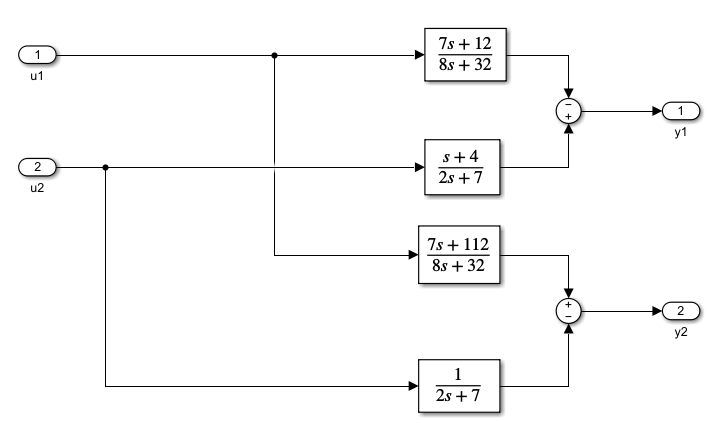
\includegraphics[width=0.6\textwidth]{scheme_task3.png}
\caption{Схема системы - MIMO, EE}
\end{figure}

\section{Графики сигналов u(t) и y(t)}
 
\begin{figure}[ht]
  \centering
  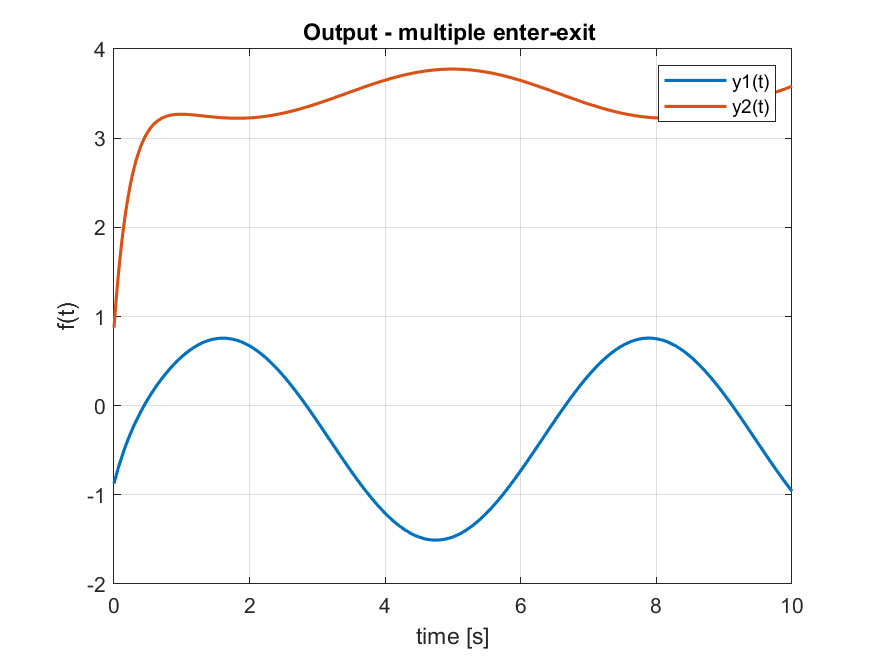
\includegraphics[width=1\textwidth]{output_task3_multiple_EE_1.png}
\caption{Симуляция - $u_1(t) = 1 , u_2(t) = 2sin(t)$}
\end{figure}

\endinput